\documentclass[11pt]{article}

\usepackage[margin=1in]{geometry}
\usepackage{amsmath, amssymb}
\usepackage{booktabs}
\usepackage{enumitem}
\usepackage{hyperref}
\usepackage{tikz}
\usetikzlibrary{positioning, arrows.meta}

\hypersetup{colorlinks=true, linkcolor=blue!50!black, urlcolor=blue!50!black, citecolor=blue!50!black}

\newcommand{\code}[1]{\texttt{#1}}

\title{SBG v2: A Tile-Native Pipeline from Real OneMap Building Meshes\\
\large to a Watertight CFD-STL}
\author{}
\date{}

\begin{document}
\maketitle

\begin{abstract}
This document describes SBG~v2, a redesigned pipeline that produces a watertight solid mesh
(STL) of a user-chosen area of Singapore --- buildings and terrain --- suitable for meshing
into a computational fluid dynamics (CFD) domain for town-scale plume dispersion modelling.
The original SBG pipeline built its buildings as flat-footprint ``extruded box'' (LoD1)
approximations and then tried to improve their heights. SBG~v2 instead takes the
\emph{real, LiDAR-surveyed building meshes} that Singapore's government 3D map (SLA OneMap~3D)
already publishes, and assembles them directly onto terrain. This document walks through what
each program in the pipeline does and the geometric processes involved --- tile fetching,
mesh extraction and reprojection, terrain draping, fusion, and watertight finishing --- as
well as the small local web application that drives it. It is deliberately light on
mathematics; it is a description of what the pipeline does and why, not a derivation.
\end{abstract}

\tableofcontents

\section{Overview}

\subsection{What changed from v1, and why}

The earlier pipeline (documented separately) reconstructed each building as a prism: a flat 2D
footprint extruded up to a single scalar height. That is an honest approximation when all you
have is a footprint and a height, but it can never represent a building whose real form is not
a uniform-height box --- towers on a podium, curved or stepped massing, and so on --- and much
engineering effort went into patching up heights that were wrong.

SBG~v2 starts from better source data. SLA's OneMap~3D service publishes the whole of Singapore
as real, surveyed building meshes, streamed as 3D~Tiles. The v2 pipeline fetches those meshes
for the requested area, places them on real terrain, and fuses the result into one watertight
solid. Buildings are no longer approximated; they are the government's own captured geometry.

\subsection{The pipeline at a glance}

Everything works in EPSG:3414 (SVY21), Singapore's official projected coordinate system, in
metres. The user draws an area on a map; the pipeline then runs six stages, each implemented by
one program:

\begin{center}
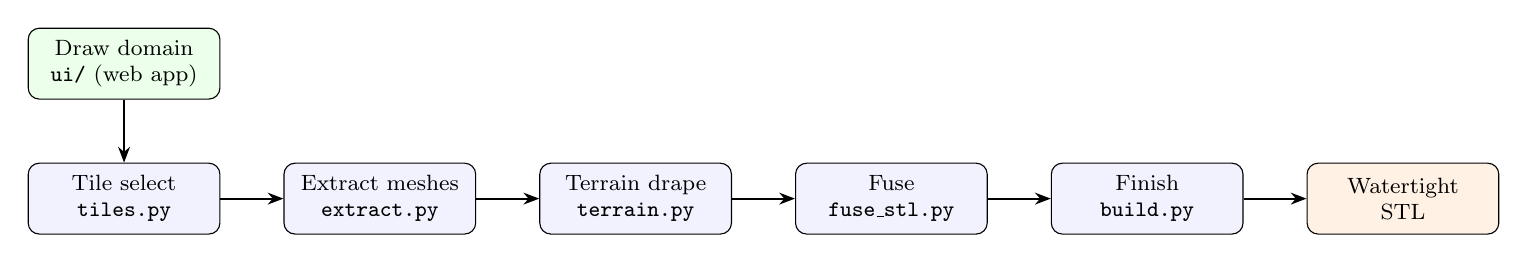
\begin{tikzpicture}[
  node distance=6mm and 8mm,
  box/.style={draw, rounded corners, align=center, font=\footnotesize,
              minimum height=9mm, text width=2.2cm, fill=blue!5},
  arr/.style={-{Stealth[length=2mm]}, thick}
]
\node[box] (tiles) {Tile select\\\code{tiles.py}};
\node[box, right=of tiles] (extract) {Extract meshes\\\code{extract.py}};
\node[box, right=of extract] (terrain) {Terrain drape\\\code{terrain.py}};
\node[box, right=of terrain] (fuse) {Fuse\\\code{fuse\_stl.py}};
\node[box, right=of fuse] (finish) {Finish\\\code{build.py}};
\node[box, above=8mm of tiles, fill=green!8, text width=2.2cm] (ui) {Draw domain\\\code{ui/} (web app)};
\node[box, right=of finish, fill=orange!10] (stl) {Watertight\\STL};
\draw[arr] (ui) -- (tiles);
\draw[arr] (tiles) -- (extract);
\draw[arr] (extract) -- (terrain);
\draw[arr] (terrain) -- (fuse);
\draw[arr] (fuse) -- (finish);
\draw[arr] (finish) -- (stl);
\end{tikzpicture}
\end{center}

The remaining sections describe each program in turn. The whole chain runs for any drawn area
in a few minutes; on a precomputed local store of decoded tiles, the fetch/extract step is
effectively instantaneous.

\section{The web application (\code{sbg.onemap\_native.ui})}
\label{sec:ui}

The pipeline is driven by a small local web app (a Python/FastAPI backend serving a Vue
frontend), launched with a single command that opens a browser tab. It is deliberately lean:
its whole job is to let a scientist define a CFD domain and get an STL back, without touching a
terminal. Its features:

\begin{itemize}[leftmargin=1.4cm]
  \item \textbf{Orientation.} A 2D top-down map of every building footprint in Singapore,
    with pan/zoom and a location search box (type a place name or coordinates to jump there).
  \item \textbf{Three ways to draw the domain boundary:} a \emph{rectangle}, a \emph{polygon}
    traced point-by-point, or a \emph{point-with-buffer} (click a location, give a radius).
  \item \textbf{Live preview.} As the boundary is drawn, buildings fully inside it are
    highlighted as ``kept'' and buildings crossing the line are highlighted as ``dropped,''
    with a running count --- so the consequence of the boundary is visible before committing.
  \item \textbf{Generate.} One button runs the whole pipeline as a background job, streaming
    its stage-by-stage progress (finding tiles, extracting, terrain, fusing, finishing) back to
    the page.
  \item \textbf{View and download.} The finished STL is rendered in an interactive 3D viewer
    for a sanity check, and downloaded with one click.
  \item \textbf{Advanced settings} (for power users): the voxel resolution, the simplification
    error tolerance, and related knobs, in a pop-up. Setting the voxel size to zero switches to
    a \emph{raw high-fidelity} mode that skips all the watertight processing and returns the
    real meshes at full detail (not watertight --- for inspection, not meshing).
\end{itemize}

The map basemap is built from an open building-footprint layer (OpenStreetMap footprints,
packaged by NUS's Urban Analytics Lab), which is separate from the OneMap meshes the STL is
actually built from --- the footprints are only used for navigation and for the in/out preview,
which is why the app starts up quickly without loading any heavy 3D data.

\section{Tile selection (\code{tiles.py})}
\label{sec:tiles}

OneMap~3D serves the country as a \emph{tileset}: a tree of tiles at increasing detail, each
tile covering a rectangular geographic region. The finest (leaf) tiles hold the real building
geometry and partition space without overlapping, so gathering every leaf tile whose region
intersects the drawn domain gives complete, non-redundant coverage of that area.

This program walks the tileset tree, pruning any branch whose bounding region does not intersect
the domain, and returns the list of intersecting leaf-tile addresses --- typically a few dozen
to a couple hundred for a town-scale domain. Each tile is then fetched, either live from the
public service (needing no local data at all, which keeps the tool portable) or from a local
copy if one has been downloaded for speed. A separate one-time job (\code{precompute.py}) can
decode every tile in the country once and cache the results, after which drawing any domain
reuses that cache instead of re-fetching.

\section{Building extraction and reprojection (\code{extract.py}, \code{transform.py})}
\label{sec:extract}

Each fetched tile is a \emph{batched} 3D model: one compressed (Draco-encoded) mesh containing
many buildings at once, plus a per-vertex integer tag (\code{\_BATCHID}) identifying which
building each triangle belongs to. This program decodes the mesh, reprojects it into Singapore
coordinates, and splits it into one piece per building.

\subsection{Getting the coordinates right}

This is the single most important step in the whole pipeline, and the one that was wrong in an
earlier attempt (with the visible result that half the area's ground came out at wildly varying
elevations). A tile's vertices are stored in a small local coordinate frame; turning a local
point $p$ into a real-world Singapore coordinate is a fixed sequence of transforms:

\begin{equation}
  p_{\text{ECEF}} \;=\; \underbrace{C}_{\text{tile centre}} \;+\; Z\big(R\,p + T\big),
  \label{eq:transform}
\end{equation}

where $R$ and $T$ are the tile's own stored rotation and translation, $Z$ is a fixed axis swap
that reconciles the 3D-model convention (``up'' is the $y$-axis) with the geographic convention
(``up'' is the $z$-axis), and $C$ is the tile's centre point in Earth-centred coordinates. The
result $p_{\text{ECEF}}$ is then converted through standard geographic transforms
(Earth-centred $\to$ latitude/longitude $\to$ SVY21). The earlier, broken version omitted the
rotation~$R$ and the axis swap~$Z$ and tried to compensate with an ad-hoc sign flip; it happened
to look correct on tiles whose rotation was near a special value and silently misplaced all the
others. With Equation~\ref{eq:transform} applied correctly, every building's base lands at a
consistent ground level with no adjustment.

\subsection{Splitting into buildings and filtering to the domain}

Using the \code{\_BATCHID} tag, the decoded mesh is separated into one piece per building. Each
piece records its triangles and a base elevation. It also records a \emph{footprint} for later
terrain placement (Section~\ref{sec:terrain}) --- but a piece's footprint is not always a single
outline. A OneMap piece occasionally spans several physically separate foundations (blocks the
survey batched together under one identifier); taking one convex hull over all of that piece's
near-base points would produce an oversized, spiky outline bridging real gaps between blocks. To
avoid that, the near-base points are grouped by simple proximity (points within about 8\,m of one
another belong to the same foundation), and one convex-hull ring is kept per real cluster,
discarding any cluster too small to be a real foundation rather than extraction noise. Most
pieces are ordinary single buildings and yield one ring; a piece spanning several disjoint blocks
yields several, each tight around its own foundation.

Two filters are applied:

\begin{itemize}[leftmargin=1.4cm]
  \item Flat, near-zero-height ``ground plate'' pieces that some tiles include are discarded ---
    they are decals, not real volume.
  \item Only buildings lying \emph{fully inside} the drawn domain are kept. A building that
    crosses the boundary is dropped in its entirety, rather than being sliced flush against the
    domain wall. This is deliberate and matches CFD practice (Section~\ref{sec:finish}): a
    building sawn off at the boundary is both physically wrong and awkward to mesh, so the
    boundary is kept in open ground.
\end{itemize}

Notably, this stage does \emph{not} try to isolate a single named building or second-guess the
tile's own geometry --- it takes the tile's real mesh as-is, exactly as OneMap's own viewer
renders it, which sidesteps a whole class of per-building matching problems that an earlier,
more clever extraction approach ran into.

\section{Terrain draping (\code{terrain.py})}
\label{sec:terrain}

OneMap models every building with its base at a single common datum (elevation zero); it carries
no per-building ground height. To sit the buildings on real terrain, this program builds a
local elevation model and places each building on a graded pad.

\subsection{The elevation model}

A digital terrain model (DTM) --- a regular grid of ground elevations --- is obtained by
cropping a precomputed, whole-island elevation grid to the domain and resampling it to the
working resolution. (That island grid was itself built once, by interpolating Singapore's sparse
20\,m-interval contour data; rebuilding it per domain is unnecessary, since terrain changes far
more slowly than anything else.) Elevation at any point between grid cells is a standard bilinear
interpolation of the four surrounding cells.

\subsection{Building compounds and flat pads}
\label{sec:compounds}

Real buildings sit on level, graded platforms, not raked to follow every undulation of the
ground. Touching or overlapping building footprints (an OneMap piece's separate foundation
clusters, or several neighbouring pieces that share a wall) are first merged into
\emph{compounds}, and every building in one compound is placed on a single shared flat pad:
\[
  z_{\text{pad}} \;=\; \operatorname{percentile}_{25}\Big(\, Z(x,y) : (x,y) \in \text{compound}\, \Big).
\]
The 25th percentile, rather than the minimum, is a deliberate choice: the underlying elevation
model is itself interpolated from sparse survey contours, and its surface is built of flat
triangular facets whose \emph{creases} can dip slightly below the true local grade. Taking the
minimum chases that one spurious dip and sinks the whole compound into a shallow pit; a low
percentile sits it at the real grade instead. Each building is then shifted vertically so its
base rests at its compound's $z_{\text{pad}}$, and is given a downward \emph{skirt} --- a short
vertical wall following its own footprint outline (not the compound's, so the skirt never crosses
the open gap between two separate foundations in the same OneMap piece), plunging a fixed depth
below the pad into the terrain slab described in Section~\ref{sec:fuse}. This guarantees the
building and the ground genuinely overlap in volume rather than merely touching at a surface, and
also fixes ``podium-tower'' developments, whose surveyed tower mesh sometimes begins several
metres up (on top of a car-park podium) and would otherwise float above the ground and be
discarded.

\subsection{Conforming terrain}
\label{sec:conforming-terrain}

An early version of this stage flattened pads directly in the elevation \emph{raster} --- setting
every grid cell under a footprint to $z_{\text{pad}}$ and leaving the rest of the grid alone. That
works for an isolated building on flat ground, but a heightfield grid cannot grade a flat pad
smoothly into a slope: at a raster's native resolution the transition is either a blocky one-cell
step, or (if softened by blending pad and slope together near the edge) an excavated moat around
every building. On real hilly terrain with several buildings close together those moats overlap
into a visible ravine cutting between the buildings --- a genuine, user-reported defect in the
first implementation of this stage.

The terrain is therefore built instead as a \emph{constrained Delaunay triangulation}, not a
raster grid. Every compound's footprint ring is inserted directly into the triangulation as a
constraint, with its vertices pinned to the compound's flat $z_{\text{pad}}$; a background grid of
points elsewhere in the domain, together with the domain boundary itself, is pinned to the real
elevation model. The triangulation connects all of this with clean triangles, which by
construction slope smoothly from a pad's edge to the surrounding real terrain --- no raster step,
no moat, and no risk of a sliver hull from one piece's footprint cutting a trench across open
ground, since the terrain now only ever gains a vertex where a real constraint (a pad edge, the
domain boundary, or a background grid point) puts one.

A compound whose own footprint spans a large elevation change (a big merged complex straddling a
hillside) would be poorly served by one shared flat pad --- its uphill half would sink into the
slope. Such a compound can instead be \emph{draped}, meaning the terrain is allowed to follow the
real elevation model through it rather than being pinned flat; each of its buildings then sits at
its own local ground elevation instead of the compound's shared pad. This is implemented but
currently unused in practice: draping removes a building's solid, flat foundation, and the
building mesh (which has no floor of its own) then rests on ground that drops away beneath part of
it, leaving a thin hollow shell that the voxel remesh step (Section~\ref{sec:fuse}) can erode away
entirely. Splitting the OneMap pieces into tight per-foundation footprint clusters
(Section~\ref{sec:extract}) already keeps ordinary compounds small enough that this is rarely
needed, so every compound is flattened for now; draping remains available as a building block for
a future per-block terrain-following scheme.

\section{Fusion into one solid (\code{blender/fuse\_stl.py})}
\label{sec:fuse}

At this point the scene is a collection of separate closed building meshes, plus an open terrain
surface. This program (which runs inside Blender's geometry engine) turns them into one solid:

\begin{enumerate}[leftmargin=1.4cm]
  \item \textbf{Solidify the terrain.} The terrain surface, so far an infinitely-thin sheet, is
    extruded downward by a fixed depth into a genuine slab with volume.
  \item \textbf{Join everything} --- terrain slab, every building, every skirt --- into a single
    mesh, overlaps and self-intersections and all. No attempt is made to compute an exact
    geometric union of the parts; a direct exact union was tried in the earlier pipeline and
    proved hopelessly fragile against this much real-world data irregularity.
  \item \textbf{Voxel remesh.} The joined ``mesh soup'' is resampled onto a regular 3D grid: each
    grid cell is classified as inside or outside the combined solid, and one clean, new,
    self-consistent surface is re-extracted from that classification. Because this step only asks
    ``is this point inside or outside?'' it does not care that its input overlaps or
    self-intersects --- which is exactly why it succeeds where an exact union fails. Its output is
    watertight by construction.
\end{enumerate}

The result is written out in a compact binary form for the finishing stage. The voxel resolution
is a chosen parameter: matching it to the resolution of the eventual CFD mesh means no real
detail is lost (the CFD mesher would discard finer detail anyway), while a needlessly fine
setting simply inflates the triangle count for no benefit.

\section{Watertight finishing (\code{build.py})}
\label{sec:finish}

The orchestrator program \code{build.py} runs all of the above and then applies the finishing
steps, all of which use a computational-geometry library whose mesh representation
\emph{cannot even express} a non-watertight defect --- so these steps preserve watertightness by
construction rather than by hoping.

\begin{enumerate}[leftmargin=1.4cm]
  \item \textbf{Simplify.} The voxel remesh tessellates flat walls and roofs just as densely as
    everything else, which is wasteful. A simplification pass collapses redundant triangles down
    to a target detail level, governed by a maximum-allowed geometric error tied to the CFD cell
    size --- so it removes triangles that carry no shape information the solver would see, while
    guaranteeing no vertex moves more than a cell's worth. This replaced an older two-tool
    approach (a separate simplifier plus a separate repair step) that could not keep the mesh
    watertight; the current single library keeps it watertight throughout.
  \item \textbf{Clip to the domain.} The mesh is intersected with a vertical prism built from the
    exact domain boundary --- a box for a rectangular domain, or the true polygon shape for a
    drawn polygon --- giving clean vertical domain walls along every edge, including concave
    corners.
  \item \textbf{Drop floating debris.} The remesh occasionally leaves a few tiny disconnected
    slivers hovering in the air (a resampling artefact, a fraction of a percent of the mesh).
    A component that is both small \emph{and} floating above the local ground is removed;
    real buildings, which sit on or into the ground, are never touched. (Verified: this leaves
    zero floating fragments while altering no real geometry.)
  \item \textbf{Polish.} A final pass removes a handful of zero-area sliver faces that would
    otherwise make a strict re-check report the mesh as non-watertight, leaving a mesh that is
    clean under the strictest interpretation --- which is what a demanding CFD mesher wants.
\end{enumerate}

The output is a single watertight STL, verified directly (holes: none; non-manifold edges: none)
rather than assumed. For inspection rather than meshing, the raw high-fidelity mode
(Section~\ref{sec:ui}) skips steps 1--4 entirely and simply exports the real meshes on terrain,
at full detail and (by design) not watertight.

\subsection{A note on the domain boundary and CFD}

Dropping whole buildings at the boundary (rather than slicing them) is not just tidier --- it is
the CFD-defensible choice. Both major solver ecosystems (ANSYS Fluent and OpenFOAM) prefer the
domain boundary to sit in open, undisturbed flow, set back from any building: a building sawn
off flush with a domain wall is unphysical at an inlet and creates coincident-face problems for
the mesher. Keeping the boundary in open ground is the standard guidance, and it is what the
full-inside filter (Section~\ref{sec:extract}) and the polygon clip produce.

\section{Running it elsewhere}

The tool is designed to move to another machine easily. It needs only a Python environment, an
install of the (free) Blender geometry engine whose location is configurable, and two small data
files (the footprint basemap and the terrain grid). It does \emph{not} need any bulk tile
archive: by default it fetches the handful of tiles a domain needs live from the public service.
A larger local cache of decoded tiles is an optional speed-up, not a requirement.

\section{Summary}

Table~\ref{tab:v2phases} lists each program and what it contributes.

\begin{table}[h]
\centering
\begin{tabular}{@{}p{3.3cm}p{5.0cm}p{5.8cm}@{}}
\toprule
\textbf{Program} & \textbf{Does} & \textbf{Key point} \\
\midrule
\code{ui/} (web app) & Draw domain, preview, generate, view, download & Rectangle / polygon / point-buffer; live in/out preview \\
\code{tiles.py} & Find and fetch the covering tiles & Live fetch (portable) or local cache (fast) \\
\code{extract.py} \newline \code{transform.py} & Decode real meshes, reproject, split per building & Correct 3D-Tiles transform; keep only fully-inside buildings \\
\code{terrain.py} & Place buildings on a graded terrain pad & Min-elevation pad + plunge skirt for solid ground contact \\
\code{fuse\_stl.py} & Solidify, join, voxel remesh & Watertight by resampling, not by exact union \\
\code{build.py} & Simplify, clip to domain, de-debris, polish & Single verified-watertight STL at CFD resolution \\
\bottomrule
\end{tabular}
\caption{SBG~v2 program summary.}
\label{tab:v2phases}
\end{table}

The through-line of the v2 design is to trade approximation for real captured geometry, and to
prefer constructions that make the goal (a watertight, correctly-placed solid) exactly true by
how the geometry is assembled --- the correct coordinate transform, the plunge-skirt overlap,
the voxel resample, the manifold-preserving simplifier --- rather than approximately true by
tuning tolerances after the fact.

\end{document}
